\documentclass[border=0.1cm, 12pt]{standalone}
\usepackage{tikz}
\usepackage{amsfonts}
\usepackage{amsmath,amssymb}
\usepackage{systeme,mathtools}
\usetikzlibrary{positioning,arrows.meta,quotes}
\usetikzlibrary{shapes,snakes}
\usetikzlibrary{bayesnet}
\tikzset{>=latex}
\tikzstyle{plate caption} = [caption, node distance=0, inner sep=0pt,
below left=5pt and 0pt of #1.south]
\begin{document}
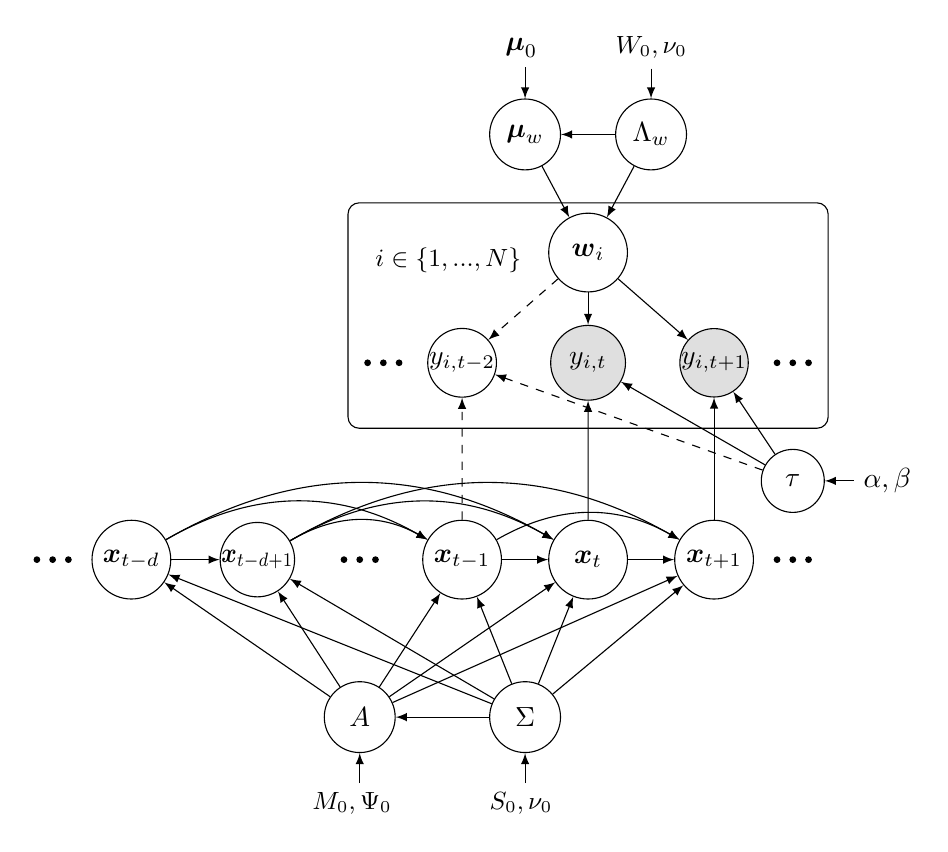
\begin{tikzpicture}
	\node [obs,inner sep=0pt,minimum size=0.8cm] (obs) at (0.8+2.4,0+0.8-0.3) {\normalsize$y_{i,t+1}$};
	\node [obs,minimum size=0.95cm] (obs1) at (-0.8+2.4,0+0.8-0.3) {\normalsize$y_{i,t}$};
	\node [circle,draw=black,fill=white,inner sep=0pt,minimum size=0.8cm] (obs2) at (-0.8+2.4-1.6,0.5) {$y_{i,t-2}$};
	\node [circle,draw=black,fill=white,inner sep=0pt,minimum size=0.8cm] (xtd1) at (-2.6,-2.0) {\scalebox{0.85}[1]{$\boldsymbol{x}_{t-d+1}$}};
	\node [circle,draw=black,fill=white,inner sep=0pt,minimum size=1cm] (xtd) at (-4.2,-2.0) {$\boldsymbol{x}_{t-d}$};
	\node [circle,draw=black,fill=white,inner sep=0pt,minimum size=1cm] (xt1) at (3.2,-2.0) {$\boldsymbol{x}_{t+1}$};
    \node [circle,draw=black,fill=white,inner sep=0pt,minimum size=1cm] (xt2) at (1.6,-2.0) {$\boldsymbol{x}_{t}$};
	\node [circle,draw=black,fill=white,inner sep=0pt,minimum size=1cm] (xt3) at (0,-2.0) {$\boldsymbol{x}_{t-1}$};
	\node [circle,draw=black,fill=white,inner sep=0pt,minimum size=1cm] (w) at (2.4-0.8,2.3-0.4) {$\boldsymbol{w}_{i}$};
    \node [circle,draw=black,fill=white,inner sep=0pt,minimum size=0.9cm] (lambda) at (3.2-0.8,3.8-0.4) {$\Lambda_{w}$};
    \node [circle,draw=black,fill=white,inner sep=0pt,minimum size=0.9cm] (mu) at (0+2.4-1.6,3.8-0.4) {$\boldsymbol{\mu}_{w}$};
    \node [circle,draw=black,fill=white,inner sep=0pt,minimum size=0.9cm] (kappa) at (0.8,-4) {$\Sigma$};
    \node [circle,draw=black,fill=white,inner sep=0pt,minimum size=0.9cm] (thetak) at (-1.3,-4) {$A$};

	\node[mark size=1pt,color=black] at (-1.6+2.4-1.6,0+0.8-0.3) {\pgfuseplotmark{*}};
	\node[mark size=1pt,color=black] at (-1.8+2.4-1.6,0+0.8-0.3) {\pgfuseplotmark{*}};
	\node[mark size=1pt,color=black] (leftnode0) at (-2.0+2.4-1.6,0+0.8-0.3) {\pgfuseplotmark{*}};

	\node[mark size=1pt,color=black] at (1.6+2.4,0+0.8-0.3) {\pgfuseplotmark{*}};
	\node[mark size=1pt,color=black] at (1.8+2.4,0+0.8-0.3) {\pgfuseplotmark{*}};
	\node[mark size=1pt,color=black] (rightnode0) at (2.0+2.4,0+0.8-0.3) {\pgfuseplotmark{*}};

	\node[mark size=1pt,color=black] at (-1.1,-2) {\pgfuseplotmark{*}};
	\node[mark size=1pt,color=black] at (-1.3,-2) {\pgfuseplotmark{*}};
	\node[mark size=1pt,color=black] at (-1.5,-2) {\pgfuseplotmark{*}};

	\node[mark size=1pt,color=black] (leftnode1) at (-5.4,-2) {\pgfuseplotmark{*}};
	\node[mark size=1pt,color=black] at (-5.2,-2) {\pgfuseplotmark{*}};
	\node[mark size=1pt,color=black] at (-5.0,-2) {\pgfuseplotmark{*}};

	\node[mark size=1pt,color=black] (rightnode1) at (4.4,-2) {\pgfuseplotmark{*}};
	\node[mark size=1pt,color=black] at (4.2,-2) {\pgfuseplotmark{*}};
	\node[mark size=1pt,color=black] at (4.0,-2) {\pgfuseplotmark{*}};

    \node [circle,draw=black,fill=white,inner sep=0pt,minimum size=0.8cm] (tau) at (3.0+2.4-1.2,-1.8+0.8) {$\tau$};
    \node [text width=0.6cm] (gamma1) at (3.0+2.4,-1.8+0.8) {$\alpha,\beta$};
    \node [text width=0.9cm] (gamma2) at (0+2.4,4.8-0.3) {\small $W_0,\nu_0$};
    \node [text width=0.5cm] (mu0) at (0+2.4-1.6,4.8-0.3) {$\boldsymbol{\mu}_0$};
    \node [text width=0.9cm] (gamma3) at (0.8,-5.1) {\small $S_0,\nu_0$};
    \node [text width=1.2cm] (gamma4) at (-1.3,-5.1) {\small $M_0,\Psi_0$};
    
    \path [draw,->] (w) edge (obs);
    \path [draw,->] (w) edge (obs1);
 	\path [draw,->,dashed] (w) edge (obs2);
    \path [draw,->] (lambda) edge (w);
    \path [draw,->] (kappa) edge (xtd);
    \path [draw,->] (kappa) edge (xtd1);
    \path [draw,->] (kappa) edge (xt1);
    \path [draw,->] (kappa) edge (xt2);
    \path [draw,->] (kappa) edge (xt3);
    \path [draw,->] (gamma1) edge (tau);
    \path [draw,->] (gamma2) edge (lambda);
    \path [draw,->] (gamma3) edge (kappa);
    \path [draw,->] (gamma4) edge (thetak);
    \path [draw,->] (lambda) edge (mu);
    \path [draw,->] (mu) edge (w);
    \path [draw,->] (mu0) edge (mu);
    \path [draw,->] (tau) edge (obs);
    \path [draw,->] (tau) edge (obs1);
    \path [draw,->,dashed] (tau) edge (obs2);
	\path [draw,->] (xt1) edge (obs);
	\path [draw,->] (xt2) edge (xt1);
 	\path [draw,->] (xt3) edge (xt2);
 	\path [draw,->,dashed] (xt3) edge (obs2);
	\path [draw,->] (xt3) edge [bend left] node [right] {} (xt1);
 	\path [draw,->] (xtd) edge [bend left] node [right] {} (xt2);
 	\path [draw,->] (xtd) edge [bend left] node [right] {} (xt3);
 	\path [draw,->] (xtd) edge (xtd1);
 	\path [draw,->] (xtd1) edge [bend left] node [right] {} (xt1);
 	\path [draw,->] (xtd1) edge [bend left] node [right] {} (xt2);
 	\path [draw,->] (xtd1) edge [bend left] node [right] {} (xt3);
	\path [draw,->] (xt2) edge (obs1);
	\path [draw,->] (thetak) edge (xt1);
	\path [draw,->] (thetak) edge (xt2);
	\path [draw,->] (thetak) edge (xt3);
	\path [draw,->] (thetak) edge (xtd);
	\path [draw,->] (thetak) edge (xtd1);
	\path [draw,->] (kappa) edge (thetak);

    \node [text width=2.2cm] (m) at (-1+2.5-1.5,2.6+0.8-1.6) {\small{$i\in\left\{1,...,N\right\}$}};
    \plate [color=black] {part1} {(leftnode0)(rightnode0)(obs)(obs1)(w)(m)} { };
\end{tikzpicture}
\end{document}